\documentclass[main.tex]{subfiles}
\begin{document}

% \section*{Thu Dec 19 2019}

% The lessons on gravitational waves will be on the 8th and 9th of January, from 14:30 to 16:30, in rooms LUF2 and P2B respectively. 

\subsection{The Chandrasekhar limit in more detail}

We want to derive the Chandrasekhar limit in a more precise manner. 

% The number density of electrions is given by 
% %
% \begin{align}
% n_e = Y_{e} \frac{\rho_c}{m_H}
% \,,
% \end{align}
% %
% in the nonrelativistic case the pressure is given by 
% %
% \begin{align}
% P_c = k _{\text{NR}} n_e^{5/3} = k _{\text{NR}} \qty(\frac{Y_e \rho_{c}}{m_H})^{5/3}
% \,,
% \end{align}
%
% but we can also derive it by 
% %
% \begin{align}
% P_c = k _{\text{NR}} n_e^{5/3} = k _{\text{NR}} \qty(\frac{Y_e \rho_{c}}{m_H})^{5/3}
% \,,
% \end{align}
% %
% and equating these we find: 
%
% \begin{align}
%  k _{\text{NR}} \qty(\frac{Y_e \rho_{c}}{m_H})^{5/3}
%  = k _{\text{NR}} n_e^{5/3} = k _{\text{NR}} \qty(\frac{Y_e \rho_{c}}{m_H})^{5/3}
% \,,
% \end{align}
% %
% which implies 
% %
% \begin{align}
% \rho_{c} = \frac{3.1}{Y_e^{5}} \qty(\frac{M}{M_{*}})^2 \frac{m_H}{(h / m_e c^2)^3}
% \,,
% \end{align}
%
% where \(\alpha_{G} = G m_H^2 / (\hbar c) \approx \SI{5.9e-30}{}\), while 
% %
% \begin{align}
% m_{*} = \alpha_{G}^{-3 /2 } m_H = 1.85 M_{\odot}
% \,,
% \end{align}
% %
% while for the ultrarelativistic case we get 
% %
% \begin{align}
% P_C = k _{\text{UR}} n_e^{4/3} = k _{\text{UR}} \qty(\frac{Y_e \rho_{c} }{m_H})^{4/3}
% \,,
% \end{align}
%
% so in this particular case the density \(\rho_{c}\) simplifies from the equations: we get a critical mass 
% %
% \begin{align}
% M _{\text{CHANDRA}} = \qty(\frac{36}{\pi })^{1/2} 
% \qty(\frac{Y_e}{m_H})^2
% \qty(\frac{k _{\text{UR}}}{G})^{3/2} \approx 
% 2.3 Y_e^2 m_{*} \approx 4.3 Y_e^2 M_{\odot}
% \,,
% \end{align}
%
% and we assume that we are in the fully degenerate case: in the integration over momenta of the phase space distribution we insert a cutoff at the Fermi energy.

% We find: 
Instead of approximating the gas as either ultrarelativistic or nonrelativistic, we can use the correct expression for the particle energy in the integral for the momentum:
%
\begin{align}
P = \frac{4 \pi }{3 h^3} g_{*} \int_{0}^{p_F} \dd{p} p^2 \frac{p^2 c^2}{\epsilon_{p}}
\,,
\end{align}
%
with \(\epsilon_{p} = \qty(p^2c^2 + m^2c^{4})^{1/2}\).

We change variables to the dimensionless \(x = p / (m_e c)\) and substitute \(g_* = 2\), since electrons have spin \(1/2\):
%
\begin{align}
P = \frac{8 \pi }{3 h^3} m_e^4 c^{5} \int_{0}^{x_F} \frac{x^{4}}{(1+x^2)^{1/2}} \dd{x}
\,.
\end{align}

The variable \(x_F\) is given by:
\begin{align}
x_F = \frac{p_F}{m_ec} = 
\qty(\frac{3 n_e}{8 \pi })^{1/3} \frac{h}{m_e c} =
\qty(\frac{3 Y_e \rho_{c}}{8 \pi m_H})^{1/3} \frac{h}{m_e c}
\,,
\end{align}
%
and, since the electrons are fully degenerate, \(x_F \gg 1 \) corresponds to the ultrarelativistic case while \(x_F \ll 1\) corresponds to the nonrelativistic case.

Now, as \(x_F \to \infty \) the integral is asymptotically 
%
\begin{align}
\int_0^{x_F} \frac{x^{4}}{\sqrt{1 + x^2}} \dd{x} \sim \frac{x_F^{4}}{4}
\,,
\end{align}
%
so we define
%
\begin{align}
I(x_F) &= \frac{4}{x_F^{4}}\int_0^{x_F} \frac{x^{4}}{(1 + x^2)^{1/2}} \dd{x} \\
&= \frac{3}{2 x^{4}} \qty( x (1+x^2)^{1/2} \qty(\frac{2x^2}{3} -1) + \log \qty(x + (1+x^2)^{1/2}))
\,,
\end{align}
%
which approaches 1 as \(x_F \to \infty \).
Then, we can write the pressure as 
%
\begin{align}
P &= \frac{8 \pi }{3 h^3} m_e^{4} c^{5} \frac{x_F^{4}}{4} I(x_F)  \\
&= k_{UR} n_e^{4/3} I(x_F)
\,.
\end{align}

We can see that this manipulation works by explicitly doing the calculation, but we can also just observe that the limiting case \(x_F \to \infty \) must reduce to the ultrarelativistic approximation, so the prefactor must be the same.

% By comparison with the ultrare
% so we get \(P = k _{\text{UR}} n_e^{4/3}I(x_F)\), where we incorporated the integral in the term \(I(x_F)\): this is given by 
%

% so if \(x_F \gg 1\) we have \(I(x_F) \sim 1\), the ultrarelativistic case,
In the nonrelativistic case, \(x_F \ll 1\), we have \(I(x_F) \sim 4 x_F / 5\), and since \(x_F \sim n_e^{1/3}\) this yields \(P \sim n_e^{5/3}\) as expected. 
This expression \emph{interpolates} between the two limits.

Then, we can apply the same reasoning as before: we compare the pressure of the Fermi gas with the prediction of the Clayton model to find
%
\begin{align}
k _{\text{UR}} \qty(\frac{Y_e \rho_{c}}{m_H})^{4/3} I(x_F)
\approx \qty(\frac{\pi }{36})^{1/3} G M^{4/3} \rho_{c}^{4/3}
\,,
\end{align}
%
so we can extract the mass: 
%
\begin{align}
M = I(x_F)^{3/2} M _{\text{Ch}}
\,,
\end{align}
%
where \(M _{\text{Ch}} \approx \SI{1.4}{M_{\odot}}\) is the Chandrasekhar mass we defined earlier.
% and the important thing is that \(x_F \propto n_e^{1/3} \propto \rho_{c}^{1/3}\). 

% [Graph: on the \(x\) axis \(M/ M _{\text{CHANDRA}}\), on the \(y \) axis \(\rho_{c}\).]
\begin{figure}[ht]
\centering
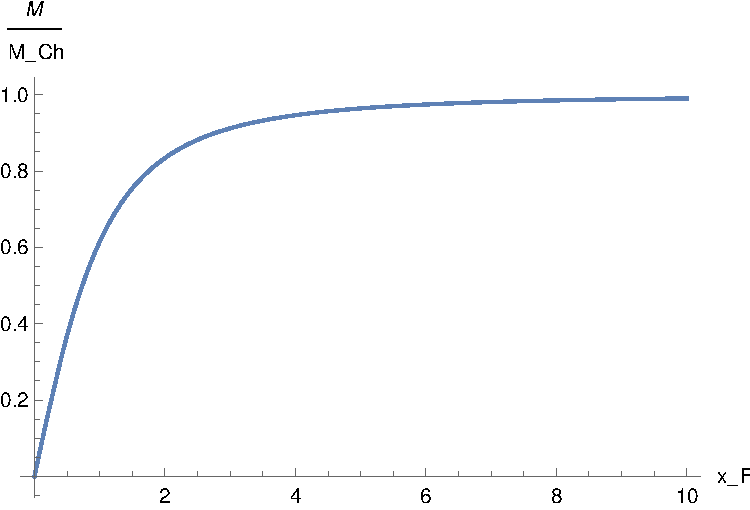
\includegraphics[width=\textwidth]{figures/chandrasekhar_limit.pdf}
\caption{A plot of \(M / M _{\text{Ch}}\) against \(x_F \propto n_e^{1/3} \propto \rho _c^{1/3}\).}
\label{chandra}
\end{figure}

\todo[inline]{Quick and dirty Mathematica plot, to update (and flip the axes maybe).}
% If we increase the mass, the star is not able to support itself by the pressure due to being a gas of degenerate electrons. 

We can see that as we increase the mass approaching \(M _{\text{Ch}}\) the central density diverges: this is not physically possible, of course, so as it gets higher some usually-prohibited process takes over; typically for white dwarfs this is electron capture, by which electrons and protons combine into neutrons, forming a neutron star.

We have not used any particular characteristics of electrons beyond their being fermions, so this line of reasoning may be used to also bound the mass of a neutron star, since neutrons are fermions as well. 
The issue, as we will see, is that general-relativistic corrections become important in that case, since neutron stars have a much higher density.

% This gives us 
% %
% \begin{align}
% M _{\text{CHANDRA }} = 3.1 Y_e^2 m_{*}
% = 5.8 Y_e^2 M_{\odot} = 1.4 M_{\odot}
% \,.
% \end{align}

\subsection{White dwarf characteristics}

% It can be shown that the mean density is around 
Now that we have a model for the equation of state at the core of a fully degenerate object like a white dwarf, we can try to extract some of its characteristics: it is reasonable (from more complete studies of the object) to estimate the mean density as 1/6 of the central one,
%
\begin{align}
\expval{\rho } = \frac{1}{6} \rho_{c}
= \frac{\num{.51}}{Y_e^2} \qty(\frac{M}{m_{*}})^2
\frac{m_H}{( h / m_e c)^3}
\,,
\end{align}
%
so we can estimate the radius as 
%
\begin{align}
R = \qty(\frac{3 M }{4 \pi \expval{\rho }})^{1/3} 
\approx \num{.77} Y_e^{5/3} \qty(\frac{M}{m_{*}})^{1/3} \underbrace{\alpha_{G}^{-1/2} \frac{h}{m_e c} }_{\ell_{WD}}
\,,
\end{align}
%
% and the object at the end is 
which is of the same order of magnitude as the characteristic length
%
\begin{align}
\ell_{WD} = \alpha_{G}^{-1/2} \frac{h}{m_e c} \approx \SI{3e7}{m} \approx \num{0.04} R_{\odot}
\,,
\end{align}
%
so, taking \(Y_e = 0.5\) we can express the radius as 
%
\begin{align}
R = \frac{R_{\odot}}{74} \qty(\frac{M_{\odot}}{M})^{1/3}
\,.
\end{align}

% The luminosity is given by 
Using the radius we can estimate the luminosity of the thermal radiation emitted by these bodies:
%
\begin{align}
L = 4 \pi R^2 \sigma T_E^{4}
= \frac{1}{74^2} \qty(\frac{M_{\odot}}{M})^{4/3}
\qty(\frac{T_E }{\SI{6000}{K}}) L_{\odot}
\,,
\end{align}
%
so if we take a typical effective temperature of around \SI{e4}{K} (recall that white dwarfs are in the blue part of the HR diagram), \(M = \num{.4} M_{\odot}\) we get \(L \approx \num{3e-3} L_{\odot}\): they are very dim. 

\subsection{Neutron stars}

The first thing to consider when discussing neutron stars is the fact that neutrons, as we discussed, are usually unstable, with lifetimes on the order of \SI{10}{min}. How can a neutron star be stable then?
% We deal with degenerate stars: the Pauli exclusion principle plays a critical role, and the process 
The process through which neutrons decay is:
%
\begin{align}
\ce{n} \rightarrow \ce{p} + \ce{e-} + \overline{\nu}_{e}
\,,
\end{align}
%
and the crucial fact is that neutron stars are composed of a degenerate neutron gas \emph{as well as} a degenerate \emph{ultrarelativistic} electron gas: the Fermi temperature is much higher than \(m_e c^2/ k_B\) \cite[eq.\ 1]{yakovlevNeutrinoEmissionNeutron}.
% When a neutron decays 
While the electron gas is ultrarelativistic the neutron gas is not; the energy released by neutron decay is of the order of \SI{800}{keV}, so the momentum an emitted electron would have would be well within the Fermi sphere, which is already full!

Thus, neutron decay is inhibited; on the other hand, electron capture, which looks like
%
\begin{align}
\ce{e-} + \ce{p} \rightarrow \ce{n} + \nu_{e}
\,,
\end{align}
%
is favoured, and it can increase the number of neutrons.

We can look at the Saha formula to get numerical estimates for the equilibrium between these processes.
The chemical potential of neutrinos can be neglected, therefore we find 
%
\begin{align}
\mu_{\ce{n}} = \mu_{\ce{p}} + \mu_{\ce{e}} 
\,,
\end{align}
%
and, since as we saw earlier the chemical potential of a Fermi gas is its Fermi energy, the same equation holds for their Fermi energies: 
% This means that a certain point we will have only neutrons. 
% We need to exploit the Fermi exclusion principle. Why does the equation 
%
\begin{align}
\epsilon_{F, \ce{n}} = \epsilon_{F, \ce{p}} + \epsilon_{F, \ce{e}}
\,.
\end{align}
%
% favour neutrons?

How does this translate into the number densities of the three constituents? We have the constraint that the number density of protons must equal the number density of electrons in order to ensure local neutrality, while there is no constraint on the ratio between neutrons and protons.
% , but the Fermi energy depends on the number density of these.
% typical numbers then become 

We will not get into the calculation, but due to the slight mass imbalance \(m_n > m_p\) we have a large difference in the number densities: typically,
%
\begin{align}
n_{\ce{p}} = n_{\ce{e}} = \frac{n_{\ce{n}}}{200}
\,.
\end{align}

% We will have 
Since the overwhelming majority of the particles in the neutron star are neutrons, we can make our calculations with the approximation that the number of neutrons per baryon is \(Y_n \approx 1\): 
%
\begin{align}
n_{\ce{n}} = Y_n \frac{\rho_{c}}{m_{\ce{n}}} \approx \frac{\rho_{c}}{m_{\ce{n}}}
\,.
\end{align}

Typical values for these densities are \(\rho_c \approx \SI{2e17}{kg/m^3}\) and \(n_{\ce{n}} \approx \SI{e44}{m^{-3}}\).

% For a neutron star we have 
With a similar reasoning to the one we applied to white dwarfs we can calculate
%
\begin{align}
\rho_{c}^{\text{NS}} \approx 3.1 \qty(\frac{M}{M_{*}})^2 \frac{m_n}{\qty(h / m_n c)^3}
\,,
\end{align}
%
% while for a white dwarf we have 
which, due to the fact that \(m_{n} \gg m_e\), is much larger than the corresponding result for white dwarfs 
%
\begin{align}
\rho_{c}^{WD} \approx \frac{3.1}{Y_e^{5}} \qty(\frac{M}{M_{*}})^2 \frac{m_H}{(h / m_e c^2)^{3}}
\,.
\end{align}
% \todo[inline]{why is the  \(c\), right?}

In both cases, we used the characteristic mass \(M_{*} = \alpha_{G}^{-3 /5 } m_n \approx 1.85 M_{\odot}\).

As we did before, knowing the central density we can estimate the average one, which then allows us to calculate the radius:
% and for the radius we get 
%
\begin{align}
R = \num{.77} \qty(\frac{M_{*}}{M})^{1/3} \alpha_{G}^{-1/2}  \frac{h}{m_n c}
\,,
\end{align}
%
where the characteristic length is given by 
%
\begin{align}
L_n = \alpha_{G}^{-1/2} \frac{h}{m_n c} \approx \SI{17}{km} \approx \frac{1}{1200} L_e
\,,
\end{align}
%
1200 times smaller than the corresponding length scale for white dwarfs (denoted with an \(e\) for ``electron degeneracy'').
% \(L_n\) is the characteristic length scale for a NS, \(L_e\) is the characteristic length for a white dwarf.

Finally, we can compute a maximum mass: \(M _{\text{max}}^{\text{NS}} = 3.1 M_{*} = 5.8 M_{\odot}\). 
% This is the mass of a star \emph{remnant}, which encompasses mass from the core only: the initial star will be much larger. 

% Can this NS become a BH? we need to compute 
We have neglected general-relativistic effects, but would they be relevant? The quantity we need to compute is the ratio of the Schwarzschild radius to the actual radius of the NS:
%
\begin{align}
\frac{R_{\text{Schw}}}{R} =
\frac{2GM}{Rc^2} \approx \num{.4} \qty(\frac{M}{M_{*}})^{4/3}
\,,
\end{align}
%
which is large, of order 1! We have not computed a minimum mass for a neutron star, but typically their mass is of the order of the Chandrasekhar mass, \(M^{NS} \approx 1.4 M_{\odot}\) because of how they form in supernovae (so, \(M / M_{*} \sim 1\)).
% qualitatively we can say that if it is too small then the degenerate electron gas may not be relativistic enough to stop neutron collapse.   
The neutron star might not be small enough to actually collapse into a black hole, but surely general relativity must be considered when describing its dynamics.
% so if the mass is large enough we can reach the critical value of \(GM / Rc^2 = 2\). 

Neutron stars were first detected as very regular radio pulses: \emph{pulsars}. These are due to the very strong (\(\sim \SI{e8}{T}\)) magnetic fields accelerating particles in beams aligned with the magnetic poles of the NS; these are not aligned with the rotation axis of the NS, so they constantly change the direction of emission, and the Earth can happen to be in this cone. 

In order to estimate how fast these pulses can be (in a classical and rough way), let us assume that the NS is rotating barely below a speed which would disintegrate it, so that its binding energy equals its rotational energy:
% We have 
%
\begin{align}
\frac{GM^2}{R^2} \approx R \omega^2 _{\text{max}}
\,,
\end{align}
%
% the maximum angular velocity which can be supported gravitationally: it comes out to be 
we can then compute the minimum period using the expression we have for the radius in terms of \(M\) and \(M_{*}\):
%
\begin{align}
\tau _{\text{min}} = \frac{2 \pi }{\omega _{\text{max}}} 
\approx 2 \pi \qty(\frac{R^3}{GM})^{1/2}
\approx 
11 \qty(\frac{M_{*}}{M}) \alpha_{G}^{-1/2} \frac{h}{m_n c^2}
\approx \num{.6} \frac{M_{*}}{M} \SI{}{ms}
\,.
\end{align}

The signals produced by pulsars are of this order of magnitude --- we have observed ``millisecond pulsars'', so NSs do indeed rotate close to these extremely high rates.

Neutron stars can also produce gravitational waves in their rotation, as long as they have a slight asymmetry (a ``mountain'', although their typical sizes are of the order of centimeters); these would have frequencies in the Hz range. We cannot detect these with ground-based detectors, but we might be able to do so with space-based ones. 
% This gives us a bound for gravitational waves of astrophysical origin. 
% \todo[inline]{no comment on the GR corrections to this formula: however I'd expect them to be significant}

\subsection{Relativistic corrections to the equation of state}

% We move on to \emph{the GR issue}. 
Black holes are objects which are so dense that their radius is smaller than the Schwarzschild radius:
%
\begin{align}
R < \frac{2GM}{c^2} = R _{\text{Sch}}
\,.
\end{align}

General Relativity predicts that when this is the case an \textbf{event horizon} form, a surface which forms a causal boundary: as is almost cliché, \emph{not even light can escape}.

Let us see how the classical description of a star fails for objects with relativistic masses.
The equation of hydrostatic balance, derived under classical assumptions, reads:
%
\begin{align}
\dv{P}{r} = - \frac{Gm \rho }{r^2}
\,.
\end{align}
%
% while the GR equations for this are the TOV equation: 

If we seek a relativistic analogue under similar assumption (spherical symmetry and equilibrium) we find the \textbf{Tolman-Oppenheimer-Volkov} equation: 
%
\begin{align}
\dv{P}{r} = - \frac{Gm  \rho }{r^2} \qty(1 + \frac{P}{\rho c^2}) \qty(1 + \frac{4 \pi r^3 P}{m c^2}) \qty(1 - \frac{2Gm}{rc^2})^{-1}
\,.
\end{align}
%

This equation is exact under the assumptions we mentioned. 
In the classical limit (\(2Gm/ c^2 \ll r\) and \(P \ll \rho c^2\)) this reduces to the classical hydrostatic balance equation.
The first correction is reminiscent of the second Friedmann equation: \emph{the pressure itself contributes to the inertia of the system}. 

Let us see how their predictions differ assuming constant density, \(\rho \equiv \rho_0 \). In the Newtonian case the mass below a radius \(r\) is given by
% If we have constant density, in the Newtonian case we get 
%
\begin{align}
m(r) = \frac{4 \pi }{3} \rho_0 r^3
\,,
\end{align}
%
% so than we can integrate and get 
using which we can integrate the hydrostatic balance equation (from the surface, where the pressure vanishes) to find:
%
\begin{align}
P(r) 
= \int_{R}^{r_0 } \underbrace{\qty(- \frac{Gm \rho }{r^2})}_{\dv*{P}{r}} \dd{r}
= \frac{2 \pi G}{3}  \rho_0^2 \qty(R^2 - r_0^2)
\,.
\end{align}
%
% where we inserted the boundary condition \(P(R) = 0\).

Then, the central pressure is given by 
%
\begin{align}
P_c^{\text{classical}} = \frac{2 \pi }{3} G \rho_0^2 R^2 = \qty(\frac{\pi }{6})^{1/3} G M^{2/3} \rho_c^{4/3}
\,.
\end{align}

Keeping the constant-density assumption, this can be done analytically in the relativistic case as well! We get 
%
\begin{align}
P(r) &= \rho_0 c^2 \qty(\frac{(1 - 2GM r^2 / R^3 c^2)^{1/2} - (1 - 2GM / Rc^2)^{1/2}}{3 \qty(1 - 2GM / Rc^2)^{1/2} - \qty(1 - 2GM r^2 / R^3c^2)^{1/2}})  \\
P_c^{\text{relativistic}} &= \rho_0 c^2 \frac{1 - \sqrt{1 - \frac{2GM}{Rc^2}}}{3 \sqrt{1 - \frac{2GM}{Rc^2}} - 1}
\,.
\end{align}

%
% \todo[inline]{Check exponents}
% so we get 
% %
% \begin{align}
% P_c = \frac{2 \pi }{3} G \rho_0^2R^2 = \qty(\frac{\pi }{6})^{1/3} GM^{2/3} \rho_{c}^{4/3}
% \,,
% \end{align}
% %
% so we can look at what happens when we consider \(r=0\): we get 
% %
% \begin{align}
% P_c = \rho_0 c^2 \qty(\frac{1 - \sqrt{1 - 2GM / Rc^2}}{3 \sqrt{1 - 2GM / Rc^2} - 1})
% \,,
% \end{align}
% %

% so we can see that the central pressure is finite as long as 
In the classical model we had a finite central pressure for each value of the mass and density; now, instead, in order for the pressure to not diverge we must require
%
\begin{align}
% \frac{2GM}{Rc^2} < \frac{8}{9}
R > \frac{9}{8} \frac{2GM}{c^2}
\,.
\end{align}
%
% which is not \(1/2\) since we have made some approximations. 

This is known as the \textbf{Buchdahl bound}; the radius of a non-black-hole (with constant density) cannot be arbitrarily close to the Schwarzschild radius, it must be at least \SI{12.5}{\percent} larger in order for the pressure to not diverge at the center.\footnote{
More stringent bounds can also be derived --- in \textcite[fig.\ 2]{lattimerNeutronStarObservations2007} a plot is shown of possible equations of state of neutron stars in a mass versus radius plane.
The bound we derived is denoted as \(P < \infty \), and we can also see a ``causality'' bound, which is related to the speed of sound in an ultrarelativistic medium.
Realistic equations of state can reach approximately \(R \gtrsim 3GM /c^2\).}

% \todo[inline]{A mass bound for neutron stars follows, both in Pacciani's notes and in the , but I don't follow the logic.}
This also yields a mass limit for neutron stars. Let us estimate the constant density \(\rho_0\) by assuming that each neutron takes up a sphere of radius its Compton wavelength: \(r_n \approx h / m_n c\), so 
%
\begin{align}
\rho_0 \approx \frac{m_n}{ \frac{4 \pi }{3} r_n^3}
\approx \frac{3 m_n^4 c^3}{4 \pi h^3}
\,.
\end{align}

A more accurate estimate would be given by \(r_n \approx \num{.7} h / m_n c\).

so that, using the fact that \(\rho_0 = M / ( 4 \pi R^3 / 3)\), we can start manipulating the Buchdahl bound:
%
\begin{align}
M &< \frac{4 c^2}{9GR} = \frac{4 c^2}{9 G} \qty(\frac{4 \pi \rho_0 }{3M})^{1/3}  \\
M^{2/3} &< \frac{4 c^2}{9G} \qty(\frac{4 \pi }{3} \frac{3 m_n^4 c^3}{4 \pi h^3})^{1/3} \\
M  &< \qty(\frac{8 \pi}{9})^{3/2} M_{*}
\,.
\end{align}

This yields a bound on the order of \(M \lesssim 5 M_{\odot}\).
% Then we have a bound 
% %
% \begin{align}

% \,,
% \end{align}
% %
% with \(f \sim 1\).
% This means than the objects becomes contained inside its Schwarzschild radius, \(R = 2GM/c^2\). 

% Tomorrow we will speak of galaxy formation. 

\end{document}